\section{Zašto je nastala SSD mreža}
\emph{Single Shot MultiBox Detector} (dalje \emph{SSD}) je mreža za detekciju i klasifikaciju kojoj je primarna svrha jednostavnost i brzina.
Prije nastanka \emph{SSD} mreže, najpoznatije mreže za isti zadatak bile su implementirane arhitekturom \emph{Region-Convolutional Neural Network} (dalje \emph{R-CNN}).
\emph{R-CNN} mreže na izlazu tipično daju set kvadrata koje opisuju objekt i klasu istog.
Klasični izlaz iz \emph{R-CNN} mreže vidljiv je na slici ~\ref{fig:ObjectDetectionOutput}.
Osim bazičnog, iz \emph{R-CNN}-a nastale su i mreže \emph{Fast(er)-R-CNN} koje dalje ubrzavaju i poboljšavaju preciznost iste arhitekture (\cite{ren2015faster}).
No, nijedna od tih nije uspjela doseći gotovo "real-time" brzinu sa značajnom preciznosču
\begin{figure}[h!]
	\centering
	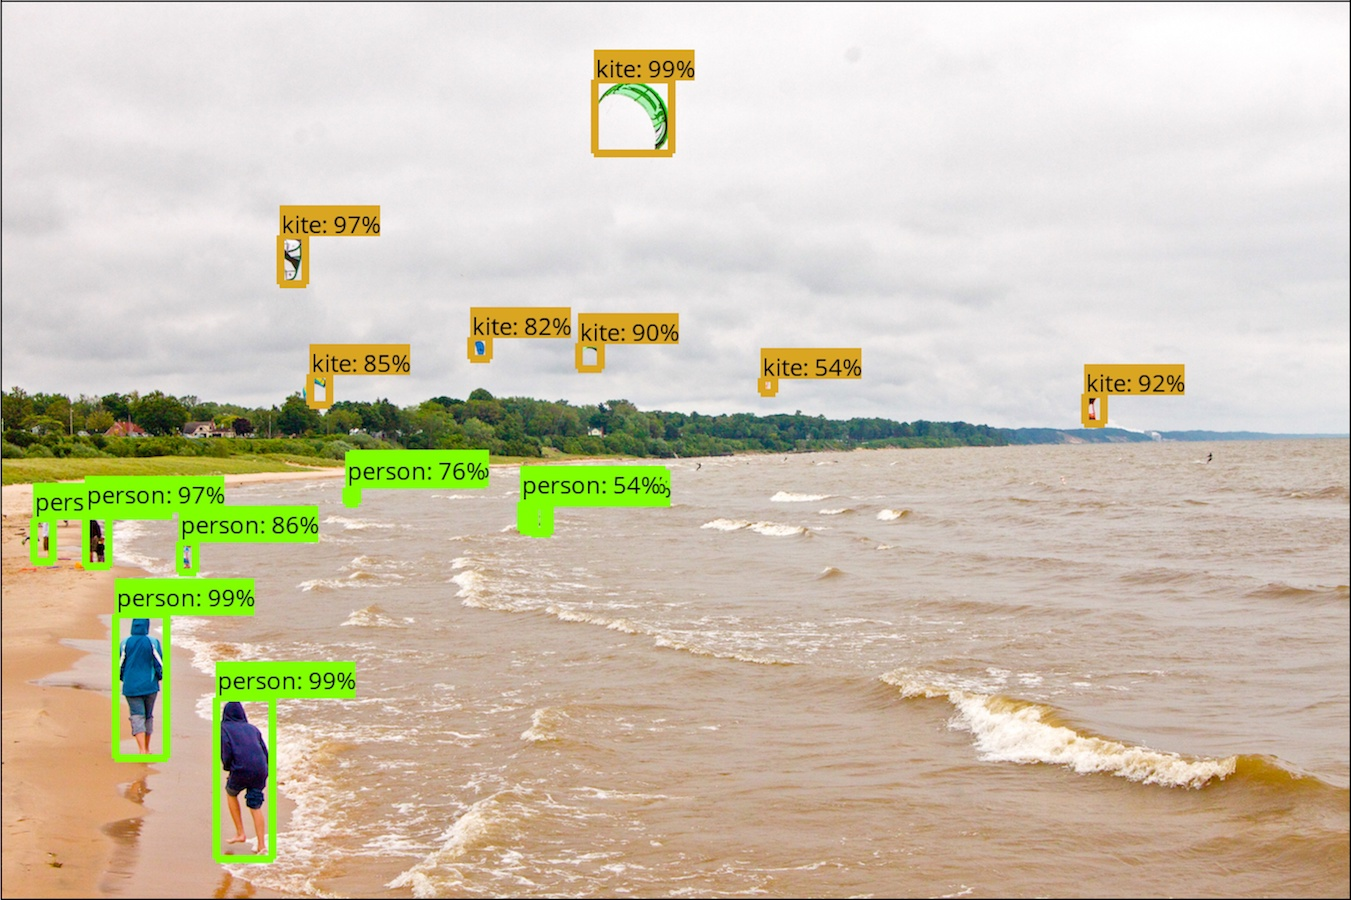
\includegraphics[width=1.0\linewidth]{object_detection_output}
	 \caption{Tipični izlaz iz mreže za detekciju i klasifikaciju sa prikazanim kvadratima i klasama}
 	 \label{fig:ObjectDetectionOutput}
\end{figure}
Iako su spomenute mreže imale pokazivale impresivne rezultate, također su imale i nekolicinu problema:
\begin{itemize}
\item Više faza treniranja
\item Komplicirana mreža
\item Mreža spora za stvarno korištenje
\end{itemize}
Zbog spomenutih problema, nastale su nove arhitekture od kojih je jedna i \emph{SSD}, koju ovaj rad koristi cjelokupnu implementaciju zadatka detekcije i klasifikacije 14 različitih klasa.

\section{Arhitektura}
\subsection{VGG-16 arhitektura}
\emph{VGG-16} je poznata neuronska mreža nastala na Oxfordu od strane \emph{Visual Geometry Group}-a, odakle i potječe ime.
Mreža sama po sebi ostvaruje odlične rezultate na \emph{ImageNet} datasetu no to nije jedini razlog zašto je jedna od najkorištenijih. \\
\emph{VGG} mreža razvijena je da bude jednostavna, sadržavajući samo \texttt{3x3} konvolucijske i \texttt{2x2} pooling slojeve prije završnih gusto spojenih slojeva (\cite{simonyan2014very}).
Arhitektura mreže vidljiva je na slici ~\ref{fig:VGGArchitecture}
Također, cijela struktura, težine i cijela istrenirana mreža je dostupna besplatno na internetu na službenoj stranici projekta (\url{http://www.robots.ox.ac.uk/~vgg/research/very_deep/}).
\begin{figure}[h!]
	\centering
	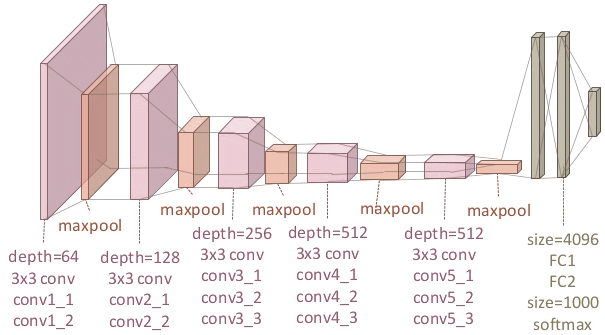
\includegraphics[width=1.0\linewidth]{vgg_architecture}
	 \caption{Arhitektura VGG-16 mreže}
 	 \label{fig:VGGArchitecture}
\end{figure}
Mana i prednost \emph{VGG-16} arhitekture je što je prostorno velika.
Oko \texttt{60MB} u svojoj cjelini sa čak \texttt{160M} parametara za treniranje što je odlična stvar za ponovno korištenje mreže za druge primjene. \\
Jedna od tih primjena je \emph{SSD} mreža, koja na svom početku sadrži baš \emph{VGG-16} arhitekturu, sve do gusto spojenih slojeva koje odbacuje.

\subsection{SSD arhitektura}
Razlog zbog kojeg \emph{SSD} mreža koristi \emph{VGG-16} kao baznu mrežu je njezina snažna performansa na slikama visoke kvalitete i popularnost gdje tehnika \emph{transfer learning}-a pomaže pri dobrim rezultatima.
Umjesto gusto spojenih slojeva \emph{SSD} mreža dodaje još konvolucijskih slojeva koji dalje izvlače značajke i progresivno smanjuju ulaz svakom dubljem sloju (\cite{liu2016ssd}).
Cijela arhitektura \emph{SSD} mreže vidljiva je na slici ~\ref{fig:SSDArchitecture}
\begin{figure}[h!]
	\centering
	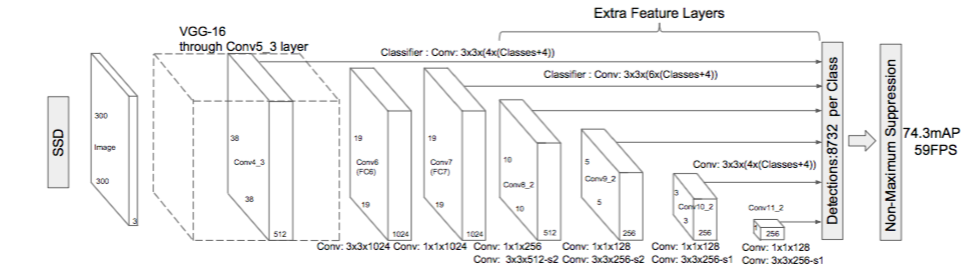
\includegraphics[width=1.0\linewidth]{ssd_architecture}
	 \caption{Arhitektura SSD mreže}
 	 \label{fig:SSDArchitecture}
\end{figure}
Slojevi dodani na baznu mrežu dodani su s ciljem da proizvedu sljedeće značajke:
\subsubsection{Detekcija značajki višestrukih veličina}
Svaki dublji konvolucijski sloj postaje manji i time promatra značajke manje veličine.
Konvolucijski model za predviđanje detekcija je drukčiji za svaki sloj.

\subsubsection{Konvolucijsko predviđanje za detekciju}
Za precizniju detekciju, različiti slojevi također prolaze kroz $3\times3$ konvoluciju kao što je prikazano na slici ~\ref{fig:SSDArchitecture}. \\
Uzmimo na primjer sloj \texttt{Conv4\_3}.
Veličina sloja je $38\times38\times512$. 
Na isti primjenjujemo konvoluciju veličine $3\times3$.
Imamo 4 kvadrata i svaki ima $klase + 4$ izlaza.
Točnije, izlaz sloja \texttt{Conv4\_3} oblika je $38\times38\times4\times(klase + 4)$. \\
U mom slučaju, to bi bilo $38\times38\times4\times(14 + 4)$ tj. $103968$ izlaza, bez računanja klasa, dobili smo $5776$ kvadrata.
Isti postupak nastavlja se dalje na dublje slojeve (\cite{ssd2}).

\section{MultiBox tehnika}
\emph{MultiBox} je tehnika za regresiju kvadrata koji ograničavaju poziciju objekta na slici.
Pretpostavljamo da smo trening podatke pripremili na način da sadrže točne koordinate kvadrata objekta.
Nakon što prođemo određeni broj konvolucija za izvlačenje značajki, dobivamo sloj veličine \texttt{mxnxp} (Slika: ~\ref{fig:SSDMultiBox}).
Za svako polje dobivamo \texttt{k} pretpostavljenih kvadrata. \\
Koncept je sljedeći. 
Uspravni kvadrat prikladan je npr. za znamenku "1" na slici, dok je za znamenku "4" ili simbol "+" prikladniji kvadrat kvadratnog oblika.
Za svaki računamo \texttt{x} vrijednosti za klase i 4 pomaka relativna originalnom, te dobivamo $(c + 4)\times k \times m \times n$ izlaza.
\begin{figure}[h!]
	\centering
	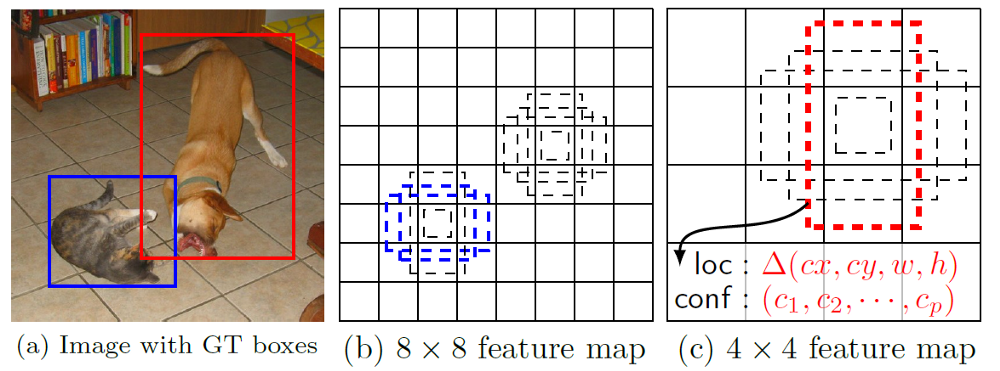
\includegraphics[width=1.0\linewidth]{ssd_multibox}
	 \caption{Višestruki kvadrati za lokalizaciju i pouzdanje}
 	 \label{fig:SSDMultiBox}
\end{figure}
Kako izračunati kvalitetu lokalizacije i pouzdanje klasifikacije? \\
\subsection{Lokalizacijski gubitak}
\emph{SSD} za izračun lokalizacijskog gubitka koristi \emph{L1-Norm}
$$|d|_\text{smooth} == \begin{cases}0.5d^2, &\text{ako}\  |d| \leq{1} \\ |d|-0.5, & \text{inače}\end{cases}$$
Iako nije precizan kao \emph{L2-Norm}, iznimno je efektivan i ispunjava svrhu \emph{SSD}-a koji se ne trudi biti točan u pixel.
\subsection{Klasifikacijski gubitak}
Za svaki dan kvadrat, \emph{SSD} vrši klasifikaciju, te računa \emph{softmax}. \\
\emph{Softmax} se koristi kao standard kada imamo više od dvije klase jer sve dobivene vrijednosti stavlja u rang $[0, 1]$ uz sumu svih koja je jednaka $1$.
$$softmax(a)=\frac{\exp{a_i}}{\sum{a_i}}$$

